\section{Introduction}
\label{sec:intro}
The Cariban language family is one of the largest of South America, with between 60'000 and 100'000 speakers unevenly distributed between 22 to 25 extant languages \parencite[441]{gildea2012classification}.
The family is concentrated in Venezuela, the Guianas and Northern Brazil, with three Western and four Southern outliers.
\cref{fig:phylomap} shows the geographical distribution and genealogical affiliation of the extant Cariban languages.
%Cariban languages feature relatively rich verbal morphology, both pre- and suffixes, inflecting for person, number, tense, aspect, and evidentiality, combined with a range of valency-modifying affixes.
%Many also have a split-\gl{s} system, which can be reconstructed to \PC \pcref{sec:split}.
For overviews of and  comparative work on the family, readers are referred to \textcites{gildea1998}{derbyshire1999carib}{meira2002first}{meira2005southern}{meira2006cariban}{gildea2007greenberg}{meira2010origin}{gildea2010story}{gildea2012classification}{matter2021cariban}{gildea2019overview}.

\begin{figure}
	\centering
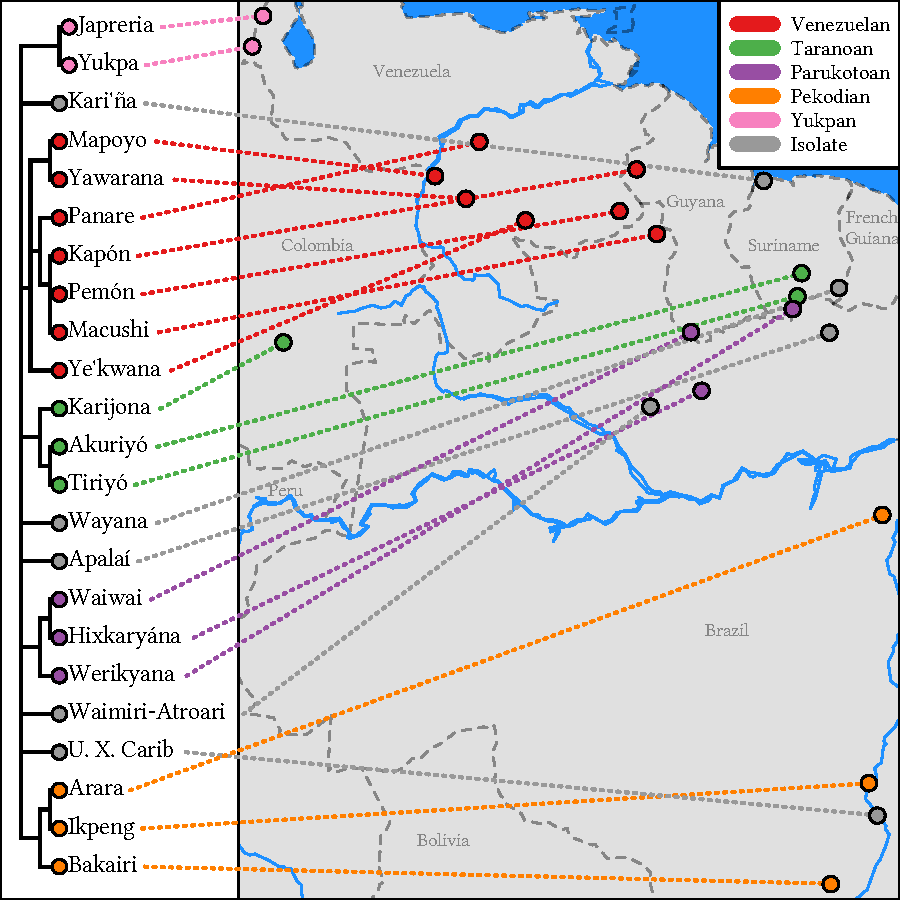
\includegraphics{floats/genealogical_map}
	\caption{The Cariban language family}
	\label{fig:phylomap}
\end{figure}

\begin{table}[htbp]
\centering
\caption[Some \hixka verbs]{Some \hixka verbs \parencites[150, 510, 511, 513, 520]{howard2001wrought}[197, 198]{hixkaryanaderby1985}}
\label{tab:hixintro}
\begin{tabular}[t]{@{}llllll@{}}
\mytoprule
{} &     \qu{to fall} &  \qu{to be afraid} &          \qu{to walk} & \qu{to cut self} &    \qu{to be} \\
\mymidrule
\gl{1}   &  \obj{k-ehurka-} &  \obj{k-oserʲehɨ-} &  \obj{k-atarʲeknohɨ-} &   \obj{k-atama-} &  \obj{w-eʃe-} \\
\gl{2}   &  \obj{m-ehurka-} &  \obj{m-oserʲehɨ-} &  \obj{m-atarʲeknohɨ-} &   \obj{m-atama-} &  \obj{m-eʃe-} \\
\gl{1+2} &  \obj{t-ehurka-} &  \obj{t-oserʲehɨ-} &  \obj{t-atarʲeknohɨ-} &   \obj{t-atama-} &  \obj{t-eʃe-} \\
\gl{3}   &  \obj{ɲ-ehurka-} &  \obj{n-oserʲehɨ-} &  \obj{n-atarʲeknohɨ-} &   \obj{n-atama-} &  \obj{n-eʃe-} \\
\mybottomrule
\end{tabular}
\end{table}
\begin{table}
\centering
\caption[Some \trio verbs]{Some \trio verbs \parencites[292, 294]{triomeira1999}[274]{triocarlin2004}}
\label{tab:triintro}
\begin{tabular}[t]{@{}llllll@{}}
\mytoprule
{} &      \qu{to sleep} & \qu{to see self} & \qu{to bathe (\gl{intr})} &     \qu{to yawn} &     \qu{to go} \\
\midrule
\gl{1}   &    \obj{t-əənɨkɨ-} &    \obj{t-əene-} &              \obj{s-epɨ-} &  \obj{s-entapo-} &  \obj{wɨ-tən-} \\
\gl{2}   &    \obj{m-əənɨkɨ-} &    \obj{m-əene-} &              \obj{m-epɨ-} &  \obj{m-entapo-} &  \obj{mɨ-tən-} \\
\gl{1+2} &  \obj{kɨt-əənɨkɨ-} &    \obj{k-əene-} &             \obj{ke-epɨ-} &  \obj{k-entapo-} &  \obj{kɨ-tən-} \\
\gl{3}   &    \obj{n-əənɨkɨ-} &    \obj{n-əene-} &              \obj{n-epɨ-} &  \obj{n-entapo-} &  \obj{nɨ-tən-} \\
\bottomrule
\end{tabular}
\end{table}

In some Cariban languages, a small group of verbs show a divergent first person inflection pattern, a topic which has not received much attention in the literature.
This is illustrated for \hixka in \cref{tab:hixintro},\footnote{All forms under discussion have prefixes from \posscite[16-18]{gildea1998} "Set I" paradigm, which is conditioned by \gl{tam} suffixes.
	The latter are omitted in tables, since a) the focus lies on the prefixes and stems, and b) full paradigms with the same \gl{tam} suffix are rare in the available sources.
Standard IPA symbols are used in the transcription languages, except for coronal rhotics of Cariban, which are simply represented with \ort{r}, rather than \ort{ɽ} for \wayana or \ort{ɾ̠} for \maqui etc.
\textcite{gildea2018reconstructing} is followed in using \ort{ə} for the \PC \rc{ô} reconstructed by \textcite{meira2005southern}, although it was likely more back \parencite{gildea2010story}.}
with paradigms of four verbs, all members of the \gl{sa} inflectional class.
In this language, the verb \qu{to be} diverges from other \gl{sa} verbs like \qu{to fall} by having a first person marker \obj{w-}, rather than \obj{k-}.
A similar pattern exists in \trio \pcref{tab:triintro}, where \gl{sa} verbs have a prefix with phonologically conditioned allomorphs \envr{\obj{t-}}{\obj{ə}} and \envr{\obj{s-}}{\obj{e}}, while the verb \qu{to go} has a first-person prefix \obj{wɨ-}.
For both languages, the first person prefix on the first four verbs in the table is representative for the vast majority of \gl{sa} verbs.
%In both languages, there are only a few other verbs inflected identically to the divergent ones on the right; for example, the first-person form of \trio \qu{to be} is \obj{w-ei-} \parencites[339]{triomeira1999}.

Such divergent verbs have been identified for \hixka \parencite[188]{hixkaryanaderby1985}, \waiwai \parencite[90]{gildea1998}, the three Taranoan languages \parencite[112--115]{meira1998proto}, \bakairi \parencite{meira2003bakairi}, and \arara \parencite[153]{alves2017arara}, but have only been subject to comparative scrutiny in \posscite{meira1998proto} reconstruction of \PTar.
In synchronic analyses, these verbs and their first person prefixes may be called \firstmention{irregular}, contrasting with regular prefixes (like \hixka \obj{kɨ-} and \trio \obj{t-}/\obj{s-}) on regular verbs.
Note that there is no widely accepted definition of irregularity \parencite{stolz2012introduction}, and many stricter definitions \parencite[e.g.,][]{haspelmath2010understanding} require the pattern to occur at a single place in the grammar.
In such approaches, these verbs simply belong to a small inflectional (sub-)class, an analysis applied to the Pekodian languages \bakairi and \arara \parencites[4]{meira2003bakairi}[149]{alves2017arara}.

Regardless of the details of synchronic analysis, the cause for the divergent inflectional patterns is found in the diachrony of the languages in question.
The goal of this study is to approach these patterns from a comparative perspective and to provide a diachronic and functional account, proceeding as follows:
In \cref{sec:background}, relevant aspects of the \PC verbal system are introduced, and it is shown that the mechanism of person marker extensions is responsible for patterns like in \cref{tab:hixintro,tab:triintro}.
In \cref{sec:data}, six incomplete person marker extensions and the verbs unaffected by them are described.
Since languages show considerable etymological overlap in their conservative verbs, these are further discussed and reconstructed.
\cref{sec:motivations} uses \posscite{bybee1985morphology} network model of morphology to search explanations for the verbs (un-)affected by each extension.
\cref{sec:discussion} summarizes and discusses the results of the study.

% analyses:
%\begin{inlinelist}
%	\item special copula prefix \parencite[188]{hixkaryanaderby1985}
%	\item inflectional subclass \parencites[149]{alves2017arara}[4]{meira2003bakairi}
%	\item \dbqu{exceptional cases} \parencite[293]{triomeira1999}
%	\item phonologically conditioned allomorphs \parencites[139]{meira2006syntactic}{meira2003primeras}[189]{hixkaryanaderby1985}
%	\item not discussed \parencites{waiwaihawkins1998}{ikpengpacheco2001}{alves2013verbo}{pacheco2003intransitivos}
%\end{inlinelist}.
%meira: non-detransitivized verbs
%alves: non-detransitivized verbs (as a consequence, o-initial)